\documentclass[UTF8,a4paper,11pt]{ctexart}
\usepackage[margin=23mm]{geometry}
\usepackage{amsmath,amssymb,booktabs,longtable,array,graphicx}
\usepackage[hidelinks]{hyperref}
\usepackage{placeins}
\graphicspath{{../../05_图片/问题一/}}
\setlength{\parindent}{2em}
\setlength{\parskip}{0.15em}
\setlength{\textfloatsep}{12pt plus 2pt minus 2pt}
\setlength{\intextsep}{10pt plus 2pt minus 2pt}
\renewcommand{\arraystretch}{1.15}
\newcolumntype{P}[1]{>{\centering\arraybackslash}p{#1\textwidth}}
\raggedbottom
\renewcommand{\topfraction}{0.95}
\renewcommand{\textfraction}{0.05}
\renewcommand{\floatpagefraction}{0.8}
\begin{document}
\section{问题一模型的建立}
\subsection{径向简化、参数与外界驱动}
将药材视为长$L=0.25\,\mathrm m$、半径$R=0.02\,\mathrm m$的均匀各向同性圆柱，研究$0\le t\le1800\,\mathrm s$内径向温度$T(r,t)$与干基含水率$C(r,t)$。其中$r$为到中心轴的距离，$C$表示单位质量干药材所含水的质量。采用固定几何与常热物性，忽略端面交换、轴向梯度、辐射、尺寸收缩与蒸发潜热，不增加温度与水分之间的交叉项。端面与侧面面积比为$R/L=0.08$，故径向近似具有几何依据，但端部局部状态不属于本模型的准确描述范围。

物性与表面交换参数均取赛题附录2，如表\ref{tab:parameter}所示。含水率依赖的扩散系数沿用题目经验关系，不进行参数拟合。附件2属于收缩情形的数据，仅核对其完整性，不进入第1问方程。
\begin{longtable}{P{0.30}P{0.22}P{0.40}}
\caption{第1问固定参数}\label{tab:parameter}\\
\toprule 参数 & 数值 & 单位\\\midrule\endfirsthead
\toprule 参数 & 数值 & 单位\\\midrule\endhead
\bottomrule\endfoot
密度$\rho$ & 820 & $\mathrm{kg/m^3}$\\
比热容$c_p$ & 2600 & $\mathrm{J/(kg\cdot K)}$\\
导热系数$k$ & 0.36 & $\mathrm{W/(m\cdot K)}$\\
换热系数$h$ & 25 & $\mathrm{W/(m^2\cdot K)}$\\
有效传质系数$h_m$ & $8\times10^{-7}$ & $\mathrm{m/s}$\\
\end{longtable}

附件1共241条数值记录，时间覆盖0至14400秒，采样间隔60秒；第1问使用0至1800秒的31个采样点。所有工作表已完整读取，未发现缺失值、非数值数据或隐藏工作表。对烘房温度$T_\infty$和浓度$C_\infty$分别做分段线性插值。若$t_j\le t\le t_{j+1}$，则
\begin{equation}
 f_\infty(t)=(1-\eta)f_j+\eta f_{j+1},\qquad
 \eta=\frac{t-t_j}{t_{j+1}-t_j},\quad f\in\{T,C\}.
\end{equation}
其中$f_j$为附件1实测环境值。所有内部时间步直接查询该插值函数，不外推、不将60秒采样值阶梯式保持。计算采用秒与米，输出位置再换算为厘米。

\subsection{温度与水分的守恒方程}
按照傅里叶定律，向径向外侧取正的导热通量为
\begin{equation}
 q_r=-k\frac{\partial T}{\partial r}.
\end{equation}
对半径$r$、厚度$\mathrm dr$的薄圆环应用能量守恒，环形体积中的储热变化等于两侧净流入热量。约去$2\pi L$并取极限，得到
\begin{equation}\label{eq:heat}
 \rho c_p\frac{\partial T}{\partial t}
 =\frac1r\frac{\partial}{\partial r}\left(rk\frac{\partial T}{\partial r}\right),\qquad 0<r<R.
\end{equation}
其中因子$r$保留圆柱不同半径处传热面积的差别。由于$k$、$\rho$和$c_p$为常数，式\eqref{eq:heat}亦可写为
\begin{equation}
 T_t=\alpha\left(T_{rr}+\frac1rT_r\right),\qquad
 \alpha=\frac{k}{\rho c_p}=1.6886\times10^{-7}\,\mathrm{m^2/s}.
\end{equation}
温度使用摄氏度；温差与开尔文温差数值相同，且本问扩散系数不含绝对温度项。

在固定干物质密度假设下，水分通量除以该密度后写为$j_r=-D(C)C_r$。对圆环应用同样的守恒关系，得到
\begin{equation}\label{eq:moisture}
 C_t=\frac1r\frac{\partial}{\partial r}\left[rD(C)C_r\right],\qquad
 D(C)=7\times10^{-9}\exp\left(-\frac{0.89}{C}\right)\,\mathrm{m^2/s}.
\end{equation}
其中指数为$-0.89/C$，已对照附录2的原始页面核实。由于$D$随$C$变化，严格展开式\eqref{eq:moisture}为
\begin{equation}
 C_t=D(C)\left(C_{rr}+\frac1rC_r\right)+D'(C)C_r^2,\qquad
 D'(C)=\frac{0.89}{C^2}D(C).
\end{equation}
因此不能将变系数方程直接替换为$D(C)$乘径向拉普拉斯算子。本研究离散未展开的通量守恒形式，避免漏掉变扩散系数的贡献。初始$D(2.55)\approx4.94\times10^{-9}\,\mathrm{m^2/s}$；干燥后$D$降低，水分向外迁移逐渐变慢。该模型的温度方程和水分方程可独立求解，不将同时计算两个场误称为双向热湿耦合。

\subsection{初始条件及表面交换条件}
初始温度与含水率均匀：
\begin{equation}
 T(r,0)=28,\qquad C(r,0)=2.55,\qquad 0\le r\le R.
\end{equation}
中心采用轴对称边界，表面采用Robin交换边界：
\begin{align}
 T_r(0,t)&=0, & C_r(0,t)&=0,\\
 -kT_r(R,t)&=h[T_s-T_\infty(t)], &
 -D(C_s)C_r(R,t)&=h_m[C_s-C_\infty(t)],\label{eq:bc}
\end{align}
其中$T_s=T(R,t)$、$C_s=C(R,t)$。烘房温度高于表面温度时，向外热通量为负，表示热量进入药材；表面浓度高于外界时，水分向外流出。中心梯度为零不意味着中心状态不随时间改变。

式\eqref{eq:bc}使用等效传质闭合：将题给烘房浓度作为表面排湿的有效外界驱动。气相湿度与药材干基含水率的质量基准不同，严格界面关系还需吸附平衡和基准转换参数；本研究不虚构这些参数，保持有效Robin关系作为既定模型假设。初始均匀含水率与瞬时开启排湿的表面通量并不相容，初始时刻之后施加交换边界，允许形成薄表层梯度，不人为改变初始数据。

\subsection{共用的守恒径向离散}
为隔离时间算法的影响，Euler与CN共用空间网格、面扩散率及端点处理。取$r_i=i\Delta r$，$i=0,\ldots,N$，$\Delta r=R/N$。节点之间的面为$r_{i+1/2}=(r_i+r_{i+1})/2$，两个外端面为0与$R$。定义节点周围小环形体积除以$2\pi L$后的权重
\begin{equation}
 w_i=\frac{r_{i+1/2}^2-r_{i-1/2}^2}{2},\quad
 w_0=\frac{\Delta r^2}{8},\quad
 w_N=\frac{R^2-(R-\Delta r/2)^2}{2}.
\end{equation}
内部节点满足$w_i=r_i\Delta r$，全部权重之和为$R^2/2$。用$(u,a,b)$统一表示两类未知量：
\begin{equation}
 (u,a,b)=\begin{cases}
 (T,\alpha,h/(\rho c_p)),&\text{温度},\\
 (C,D(C),h_m),&\text{含水率}.
 \end{cases}
\end{equation}
相邻节点的面扩散率采用算术平均$a_{i+1/2}=(a_i+a_{i+1})/2$。定义带径向面积因子的梯度通量$G$，其正向与物理向外通量相反：
\begin{align}
 G_{i+1/2}&=r_{i+1/2}a_{i+1/2}\frac{u_{i+1}-u_i}{\Delta r},\\
 G_{-1/2}&=0,\qquad G_{N+1/2}=Rb(u_\infty-u_N),\\
 \dot u_i&=F_i(\boldsymbol u,t)=\frac{G_{i+1/2}-G_{i-1/2}}{w_i}.\label{eq:semidiscrete}
\end{align}
此形式使内部相邻面的通量在求和时严格抵消。对常数扩散率，内部节点等价于圆柱坐标下的中心差分。

中心节点通过$w_0$自动得到无奇点的更新率，表面节点保留外侧半网格的储热或储水项：
\begin{align}
 F_0&=\frac{4a_{1/2}}{\Delta r^2}(u_1-u_0),\\
 F_N&=\frac{1}{w_N}\left[Rb(u_\infty-u_N)-
 \frac{r_{N-1/2}a_{N-1/2}}{\Delta r}(u_N-u_{N-1})\right].
\end{align}
表面公式体现空气交换与向内层传递之间的收支，不强制将表面状态赋值为烘房状态。在初始薄边界层尚未被网格解析时，全时空最大误差不必呈现理想二阶空间收敛。

\subsection{Euler与CN时间推进}
\subsubsection{显式Euler对照}
对式\eqref{eq:semidiscrete}使用当前时刻的变化率：
\begin{equation}
 \boldsymbol u^{n+1}=\boldsymbol u^n+\Delta t\,\boldsymbol F(\boldsymbol u^n,t_n).
\end{equation}
每步先计算全部新值，再整体替换旧数组，不在循环中混用新旧节点值。将$F_i$写为邻点输入减去$s_i u_i$，代码逐步检查$\Delta t\max_i s_i\le1$，其中$s_i$包含表面对流损失。中心热方程的限制为
\begin{equation}
 \Delta t\le\frac{\Delta r^2}{4\alpha}.
\end{equation}
对照计算取$N=40$、$\Delta r=0.5\,\mathrm{mm}$、$\Delta t=0.25\,\mathrm s$，最大损失系数为0.675422，满足凸组合条件。Euler方法的时间精度为一阶。

\subsubsection{以CN为主的隐式计算}
CN采用时间区间两端变化率的平均值：
\begin{equation}\label{eq:cn}
 \boldsymbol u^{n+1}=\boldsymbol u^n+
 \frac{\Delta t}{2}\left[\boldsymbol F(\boldsymbol u^n,t_n)+
 \boldsymbol F(\boldsymbol u^{n+1},t_{n+1})\right].
\end{equation}
对线性温度方程，令$\boldsymbol F=A\boldsymbol T+\boldsymbol s(t)$，其中$A$包含内部导热和表面换热损失，$\boldsymbol s$只包含外界驱动，得到
\begin{equation}
 \left(I-\frac{\Delta t}{2}A\right)\boldsymbol T^{n+1}
 =\left(I+\frac{\Delta t}{2}A\right)\boldsymbol T^n
 +\frac{\Delta t}{2}\left[\boldsymbol s(t_n)+\boldsymbol s(t_{n+1})\right].
\end{equation}
矩阵为三对角矩阵，采用追赶法求解，每步工作量随节点数线性增加。对角损失与环境驱动均按CN处理，不能只升级内部节点而在边界保留旧时刻输入。

对非线性水分方程，初猜$\boldsymbol C^{n+1,(0)}=\boldsymbol C^n$，每轮由当前猜测计算$D$及三对角矩阵$A^{(m)}$，求解
\begin{equation}
 \left(I-\frac{\Delta t}{2}A^{(m)}\right)\boldsymbol C^{n+1,(m+1)}
 =\boldsymbol C^n+\frac{\Delta t}{2}\boldsymbol F(\boldsymbol C^n,t_n)
 +\frac{\Delta t}{2}\boldsymbol s_C(t_{n+1}).
\end{equation}
重新使用更新后的浓度计算非线性残差
\begin{equation}
 \boldsymbol{\mathcal R}=\boldsymbol C^{n+1}-\boldsymbol C^n-
 \frac{\Delta t}{2}\left[\boldsymbol F(\boldsymbol C^n,t_n)+
 \boldsymbol F(\boldsymbol C^{n+1},t_{n+1})\right].
\end{equation}
迭代停止须同时满足更新量无穷范数小于$10^{-11}$及$\|\boldsymbol{\mathcal R}\|_\infty<10^{-12}$，最多迭代30次，失败即报错。本次每步最多4次即收敛。使用旧时刻浓度将$D$冻结一整步并不自动保持非线性方法二阶精度，因此采用上述迭代而不作该简化。

为处理初始排湿不相容性，CN的第一个完整时间步用两个后向Euler半步启动，温度和水分一致处理，后续全部使用式\eqref{eq:cn}。本文简称CN时包含此启动措施。CN在线性扩散情形的稳定性不意味着任意大步长下都保持单调，因此仍核查正值、有界性及时间收敛。

\subsection{数值验证与方法比较}
\begin{longtable}{P{0.28}P{0.14}P{0.14}P{0.14}P{0.14}}
\caption{算法配置与本次运行时间}\label{tab:method}\\
\toprule 方法 & 节点数 & 步长/s & 耗时/s & 最多迭代\\
\midrule\endfirsthead
\toprule 方法 & 节点数 & 步长/s & 耗时/s & 最多迭代\\
\midrule\endhead
\bottomrule\endfoot
Euler对照 & 41 & 0.25 & 0.381 & 0\\
CN同网格对照 & 41 & 0.25 & 2.039 & 3\\
CN主结果 & 81 & 0.25 & 2.841 & 4\\
\end{longtable}
\begin{longtable}{P{0.42}P{0.25}P{0.25}}
\caption{CN相邻分辨率全时空最大差异}\label{tab:convergence}\\
\toprule 比较 & 温度差/摄氏度 & 含水率差/(kg/kg)\\
\midrule\endfirsthead
\toprule 比较 & 温度差/摄氏度 & 含水率差/(kg/kg)\\
\midrule\endhead
\bottomrule\endfoot
时间：1与0.5秒 & 0.0000281 & 0.0000599\\
时间：0.5与0.25秒 & 0.0000060 & 0.0000150\\
空间：21与41节点 & 0.0014692 & 0.0467117\\
空间：41与81节点 & 0.0003679 & 0.0243699\\
\end{longtable}

同网格同时间步的算法对比使用41个节点、$\Delta t=0.25$秒。表\ref{tab:method}报告真实运行时间与迭代次数；运行时间仅包括推进及检查，不包含读表、绘图和Excel导出。CN每步求解方程组并作非线性迭代，故这一小规模同时间步比较中耗时高于Euler，不能宣称其必然更快。CN的价值在于二阶时间推进和放宽显式稳定步长约束。

算法差异定义为相同网格、相同每秒输出位置的最大绝对差：
\begin{equation}
 \delta_u=\max_{n,i}|u_{i,\mathrm{Euler}}^n-u_{i,\mathrm{CN}}^n|.
\end{equation}
本次温度差为$4.7798\times10^{-4}$摄氏度，含水率差为$2.8152\times10^{-4}\,\mathrm{kg/kg}$，随时间变化见图\ref{fig:method}。这些数值是算法之间的差异，不是相对解析解或实测值的误差。
\begin{figure}[htbp]\centering
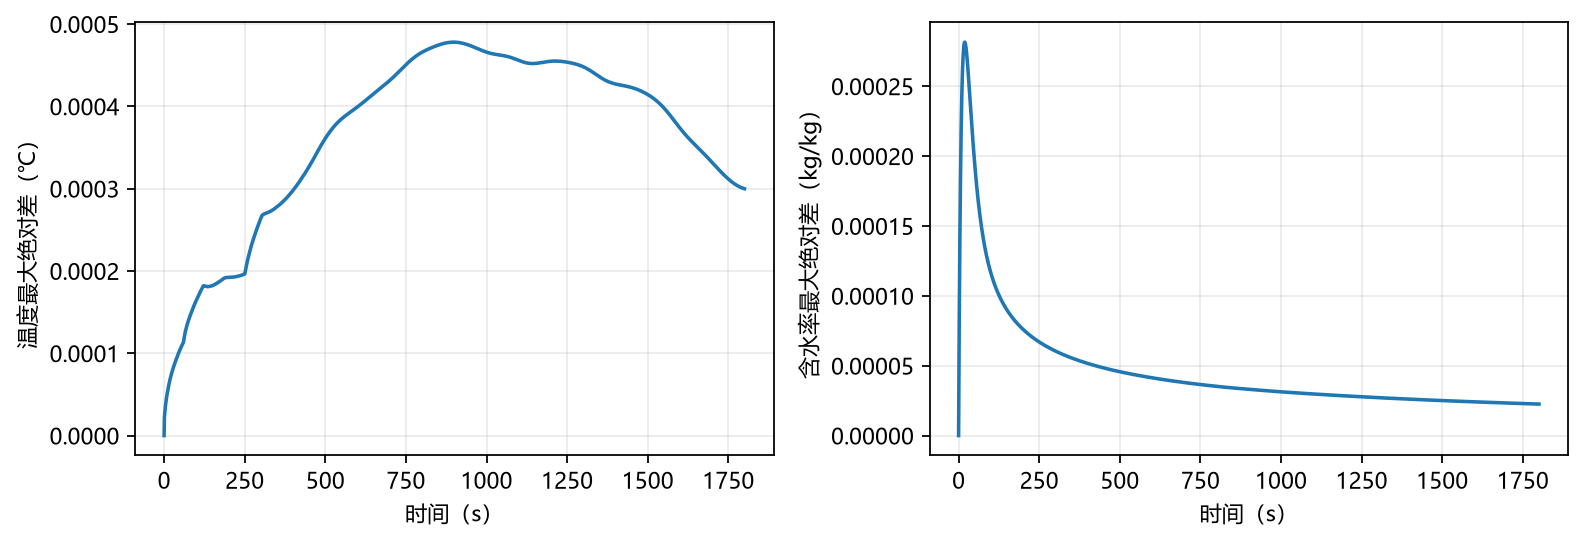
\includegraphics[width=0.98\textwidth]{Euler与CN差异.png}
\caption{相同41节点与0.25秒步长下Euler与CN的差异}\label{fig:method}
\end{figure}

时间检查固定41节点，分别使用1、0.5、0.25秒；空间检查固定0.25秒，分别使用21、41、81节点。仅在共同半径位置和共同每秒输出时刻比较，比较范围包含初始排湿阶段。差异见表\ref{tab:convergence}和图\ref{fig:convergence}。时间步连续减半后，温度相邻差异约缩小4.72倍，含水率约缩小4.00倍，支持本次时间离散的二阶趋势。
\begin{figure}[htbp]\centering
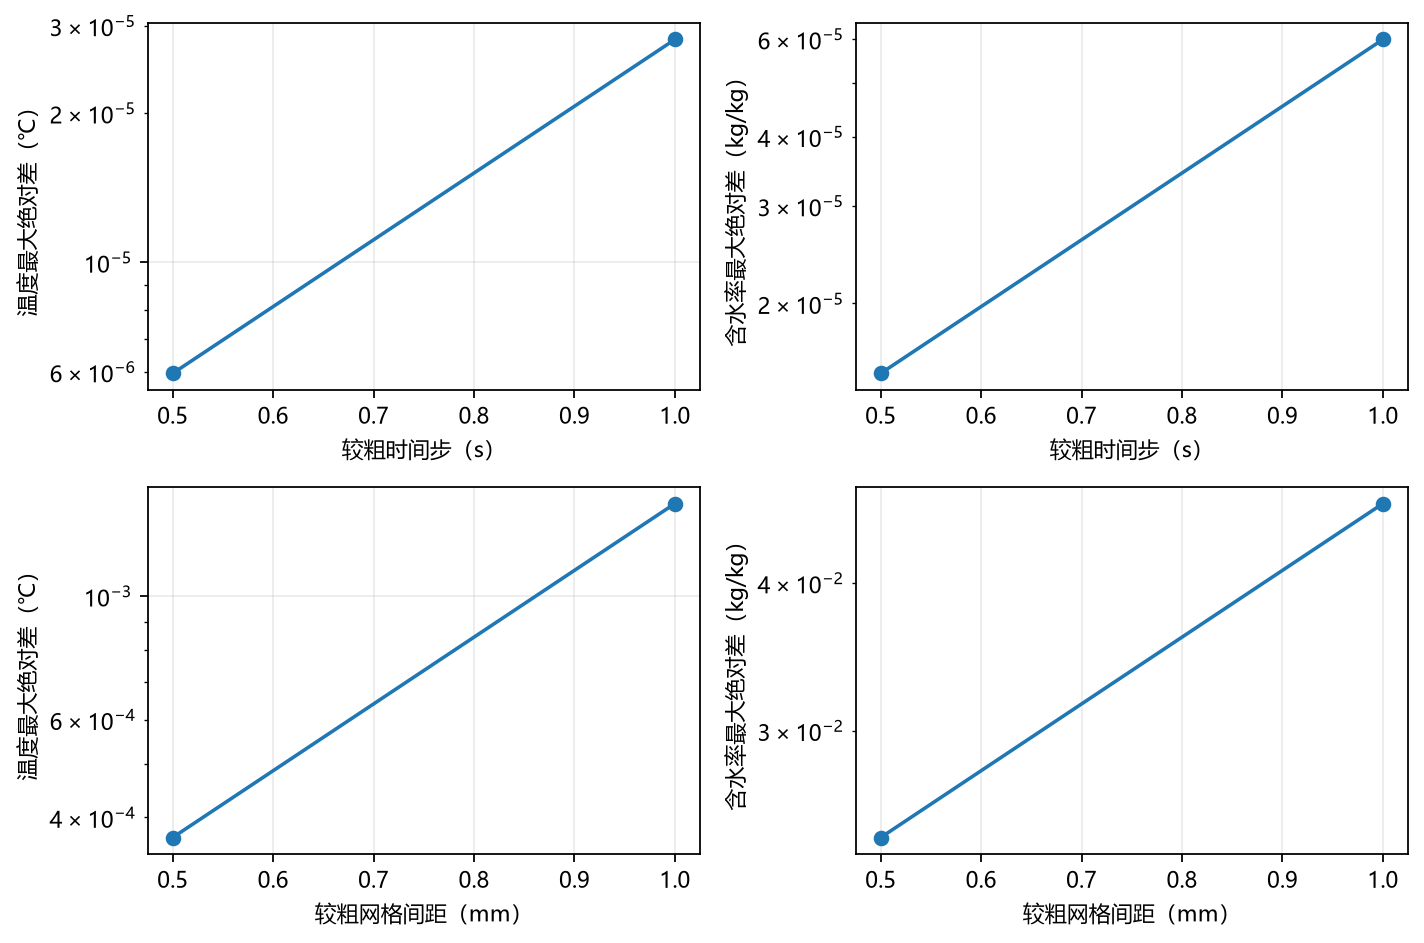
\includegraphics[width=0.86\textwidth]{收敛检查.png}
\caption{CN相邻时间步及相邻空间网格的最大差异}\label{fig:convergence}
\end{figure}

空间加密使温度差异约缩小4倍，但含水率全时空差异仅缩小约1.92倍。原因分析是初始开启排湿时形成的薄表层梯度与初始边界不相容使最大范数对早期表面状态敏感；本次检查不足以证明含水率全时空二阶空间收敛。41节点CN与81节点CN的最大含水率差仍为0.02437，尚不支持四位小数的数值精度结论。81节点结果仅作为本次较细数值参考，不是精确解；Euler与该参考的差异甚至可能因误差抵消而略小，不能据此否定或夸大任一算法。

程序还检查了全时域有限值、浓度正值、温度和含水率的径向次序及时间趋势。考虑舍入误差，单调性容差为$10^{-9}$，原始检查数值保存在JSON中。对每步离散收支，采用与相应时间格式一致的边界通量权重，得到
\begin{equation}
 \sum_iw_i(u_i^{n+1}-u_i^n)=\Delta t\left[(1-\theta)G_{N+1/2}^n+
 \theta G_{N+1/2}^{n+1}\right],
\end{equation}
其中Euler取$\theta=0$、CN取$1/2$、启动半步取1。主结果每步每单位长度热量收支最大残差约$5.42\times10^{-12}\,\mathrm{J/m}$，含水率加权平均收支残差约$1.48\times10^{-16}$。另将追赶法与小规模NumPy稠密求解独立对照，并检查均匀平衡场的右端为零，均通过$10^{-12}$容差。守恒与趋势验证不替代实验验证。
\FloatBarrier

\subsection{第1问温湿场与指定点结果}
以81节点、$\Delta t=0.25$秒的CN结果作为第1问主输出。热场与水分场分别见图\ref{fig:heat}和图\ref{fig:moisture}，各时刻径向分布见图\ref{fig:profile}。热量从表面向内部传播，表面温度始终较高；表面先排湿，中心含水率在30分钟内只发生很小变化。
\begin{figure}[!htbp]\centering
\begin{minipage}{0.49\textwidth}\centering
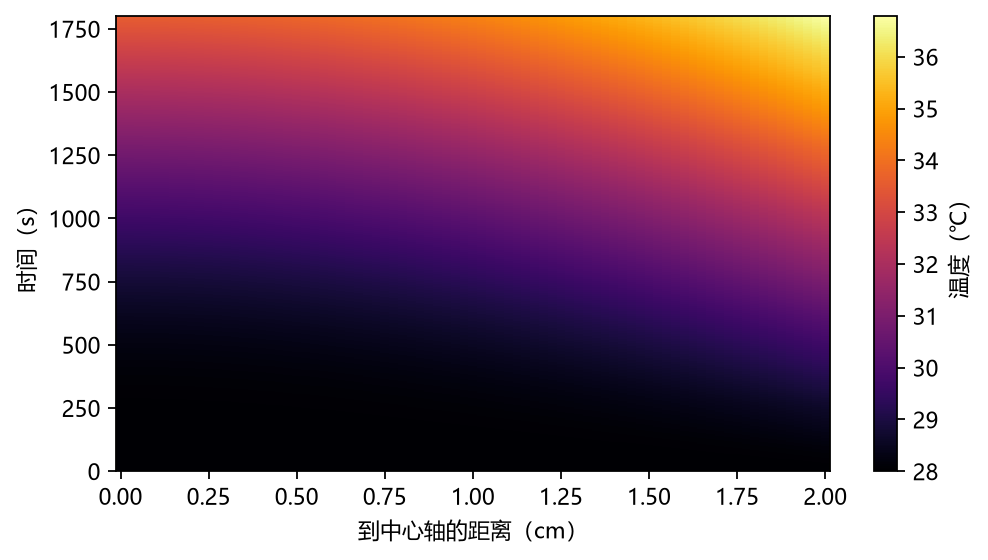
\includegraphics[width=\linewidth]{温度时空分布.png}
\caption{CN计算的径向温度场}\label{fig:heat}
\end{minipage}\hfill
\begin{minipage}{0.49\textwidth}\centering
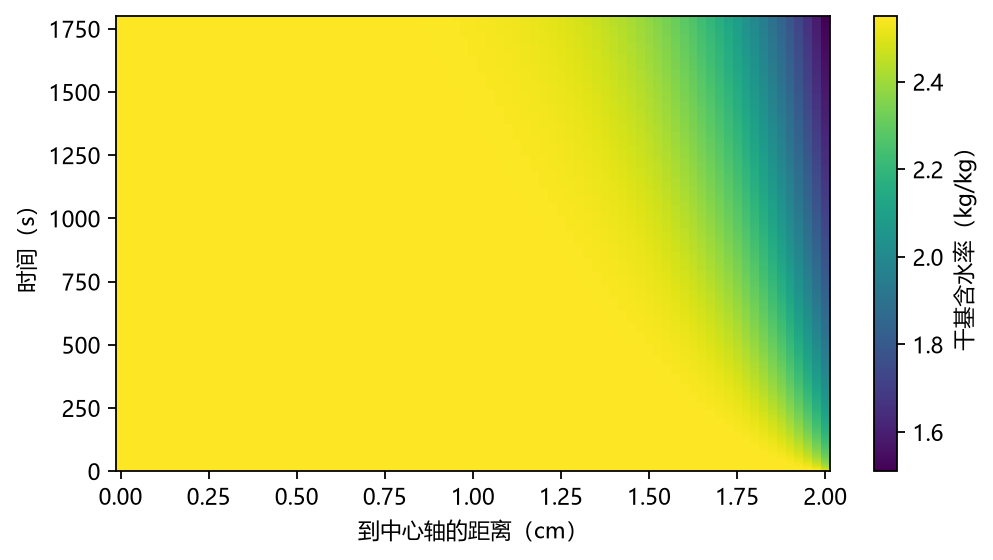
\includegraphics[width=\linewidth]{水分时空分布.png}
\caption{CN计算的径向含水率场}\label{fig:moisture}
\end{minipage}
\end{figure}
\begin{figure}[htbp]\centering
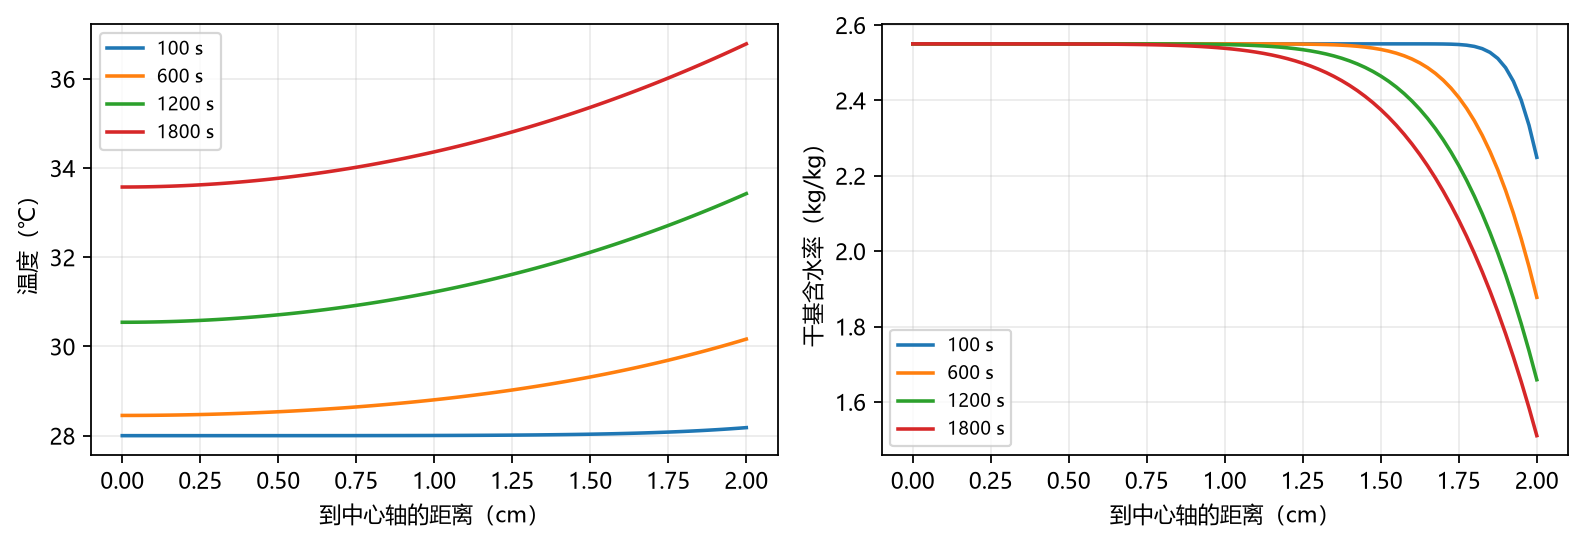
\includegraphics[width=0.98\textwidth]{径向剖面.png}
\caption{不同时刻温度与含水率的径向剖面}\label{fig:profile}
\end{figure}
\FloatBarrier
\begin{longtable}{P{0.1}P{0.14}P{0.14}P{0.14}P{0.14}P{0.14}}
\caption{指定时刻药材温度（摄氏度）}\label{tab:temperature}\\
\toprule 时间/s & 0 cm & 0.5 cm & 1 cm & 1.5 cm & 2 cm\\
\midrule\endfirsthead
\toprule 时间/s & 0 cm & 0.5 cm & 1 cm & 1.5 cm & 2 cm\\
\midrule\endhead
\bottomrule\endfoot
100 & 28.0001 & 28.0003 & 28.0041 & 28.0327 & 28.1800\\
300 & 28.0408 & 28.0635 & 28.1514 & 28.3680 & 28.8487\\
600 & 28.4534 & 28.5360 & 28.8039 & 29.3159 & 30.1652\\
900 & 29.3243 & 29.4583 & 29.8754 & 30.6161 & 31.7304\\
1200 & 30.5427 & 30.7098 & 31.2223 & 32.1125 & 33.4276\\
1500 & 31.9957 & 32.1867 & 32.7660 & 33.7463 & 35.1203\\
1800 & 33.5753 & 33.7720 & 34.3642 & 35.3621 & 36.7855\\
\end{longtable}
\begin{longtable}{P{0.1}P{0.14}P{0.14}P{0.14}P{0.14}P{0.14}}
\caption{指定时刻药材干基含水率（kg/kg）}\label{tab:moisture}\\
\toprule 时间/s & 0 cm & 0.5 cm & 1 cm & 1.5 cm & 2 cm\\
\midrule\endfirsthead
\toprule 时间/s & 0 cm & 0.5 cm & 1 cm & 1.5 cm & 2 cm\\
\midrule\endhead
\bottomrule\endfoot
100 & 2.5500 & 2.5500 & 2.5500 & 2.5500 & 2.2489\\
300 & 2.5500 & 2.5500 & 2.5500 & 2.5492 & 2.0517\\
600 & 2.5500 & 2.5500 & 2.5500 & 2.5352 & 1.8774\\
900 & 2.5500 & 2.5500 & 2.5497 & 2.5045 & 1.7550\\
1200 & 2.5500 & 2.5500 & 2.5482 & 2.4646 & 1.6588\\
1500 & 2.5500 & 2.5499 & 2.5445 & 2.4206 & 1.5789\\
1800 & 2.5500 & 2.5497 & 2.5383 & 2.3755 & 1.5103\\
\end{longtable}

表\ref{tab:temperature}和表\ref{tab:moisture}列出题目要求的7个时刻、5个半径位置，统一保留四位小数。1800秒时烘房温度为$41.5130\,{}^\circ\mathrm C$，中心与表面温度分别为$33.5753$和$36.7855\,{}^\circ\mathrm C$；中心与表面含水率分别为$2.5500$和$1.5103\,\mathrm{kg/kg}$。中心未舍入含水率为2.54999188，显示2.5500不代表其变化严格为零。

按权重计算截面平均含水率
\begin{equation}
 \overline C(t)=\frac{\sum_iw_iC_i(t)}{R^2/2},
\end{equation}
其1800秒结果为$2.2935\,\mathrm{kg/kg}$，相对初值下降约$10.06\%$。初始水分扩散尺度$\sqrt{D(2.55)\,1800}\approx3\,\mathrm{mm}$远小于20毫米半径，与短时间内中心变化较小的结果一致。主要位置随时间的变化见图\ref{fig:time}。
\begin{figure}[htbp]\centering
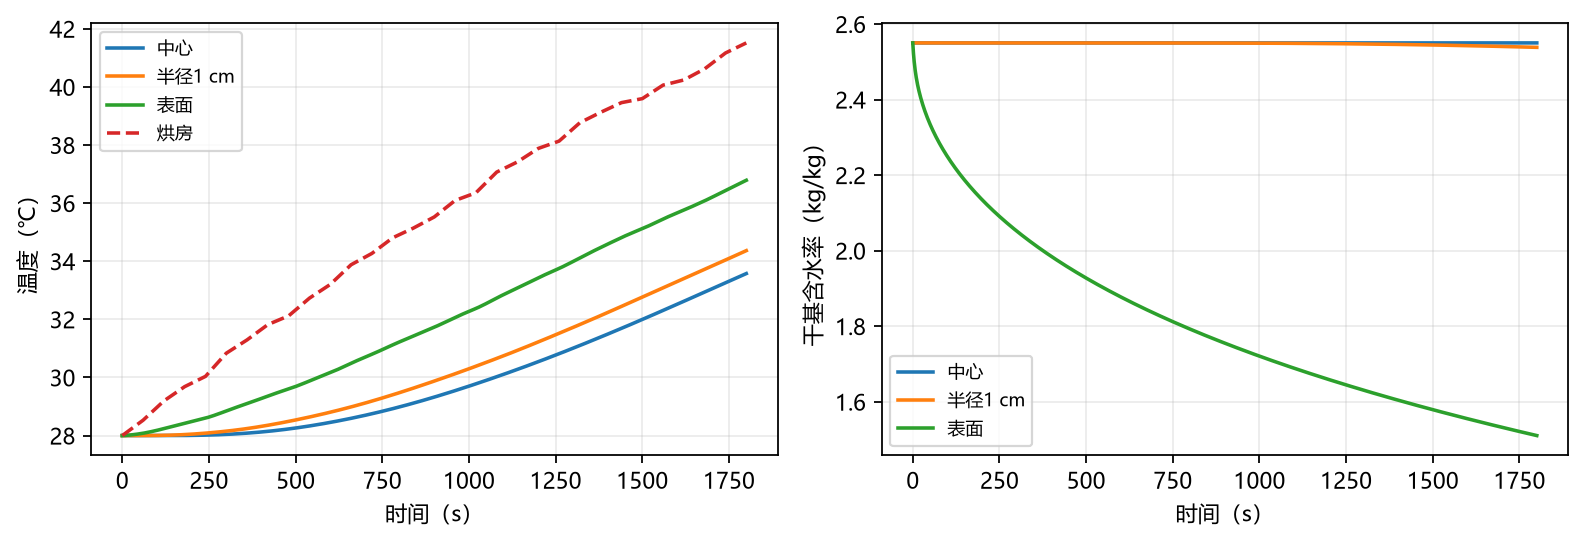
\includegraphics[width=0.98\textwidth]{时间变化.png}
\caption{中心、半径1厘米及表面的温湿变化}\label{fig:time}
\end{figure}
\FloatBarrier

烘房在该时段持续升温，内部温度随之上升并滞后，但尚未达到热平衡。因此不能把“温差必须随时间单调缩小”作为正确性的判据。结果文件按用户最新提供的附件3模板保留“温度”和“水分浓度”两表，A列为1至1800秒，首行为0至2厘米且间距0.1厘米；计算细网格直接抽取对应节点，不对空间结果再次拟合。初始0秒与未舍入全场保存在数值文件中。四位小数属于题目输出格式，本次有限收敛检查不保证每个输出的第四位均已收敛。

模型误差与离散误差须区分：继续细化网格或时间步只能改善既定方程的求解，无法消除忽略端面、潜热和气固平衡转换造成的物理近似。本问保持这些物理假设不变，以避免将算法比较混同为物理模型变化。
\end{document}
